\begin{center}
	\begin{tabular}{M{6.5cm}M{11cm}}
		\textbf{TRUNG TÂM MANABIE}& \textbf{ĐỀ ĐÁNH GIÁ NĂNG LỰC ỨNG VIÊN}\\
		\textbf{MÃ ĐỀ: DGNL24}& \textbf{Bài thi môn: VẬT LÝ}\\
		\textit{(Đề thi có 06 trang)}& \textit{Thời gian làm bài: 50 phút, không kể thời gian phát đề}
		
		\noindent\rule{2cm}{0.8pt} \\
	\end{tabular}
\end{center}
\setcounter{section}{0}
\section{Câu trắc nghiệm nhiều phương án lựa chọn}
\textit{Ứng viên trả lời từ câu 1 đến câu 20. Mỗi câu hỏi ứng viên chọn một phương án}
\setcounter{ex}{0}
\Opensolutionfile{ans}[ans/DGNL-TN]

% ===================================================================
\begin{ex}
	Trong các nhận định sau đây về kết quả thí nghiệm tán xạ của hạt alpha lên lá vàng mỏng, có bao nhiêu nhận định đúng?	
	\begin{enumerate}[label=(\arabic*)]
		\item Phần lớn các hạt alpha xuyên thẳng qua lá vàng mỏng.
		\item Một tỉ lệ khá lớn các hạt alpha bị lệch khỏi hướng ban đầu với góc lệch lớn hơn $\SI{90}{\degree}$.
		\item Một tỉ lệ rất nhỏ các hạt alpha bị lệch khỏi hướng ban đầu với góc lệch lớn hơn $\SI{90}{\degree}$.
		\item  Một số ít hạt alpha bị lệch khỏi phương ban đầu với những góc lệch khác nhau.
	\end{enumerate}
	\choice
	{1}
	{2}
	{\True 3}
	{4}
	\loigiai{
		Các nhận định đúng là: 1, 3 và 4.	
	}
\end{ex}
% ===================================================================
\begin{ex}
	Công suất của nguồn điện được xác định bằng
	\choice
	{lượng điện tích mà nguồn điện sinh ra trong một giây}
	{công mà lực lạ thực hiện được khi nguồn điện hoạt động}
	{\True công của dòng điện trong mạch kín sinh ra trong một giây}
	{công làm dịch chuyển một đơn vị điện tích dương}
	\loigiai{}
\end{ex}
%============================================================
\begin{ex}
	Hai dây dẫn thẳng, dài, đặt vuông góc với nhau, rất gần nhau nhưng không chạm vào nhau. Dòng điện qua hai dây dẫn có chiều như hình vẽ và có cùng cường độ. Từ trường do hai dây dẫn gây ra có thể triệt tiêu nhau trong vùng nào?
	\begin{center}
		\includegraphics[width=0.3\linewidth]{../figs/VN12-Y24-PH-SYL-017P-8}
	\end{center}
	\choice
	{vùng A và D}
	{\True vùng A và C}
	{vùng B và D}
	{vùng B và C}
	\loigiai{}
\end{ex}
% ===================================================================
\begin{ex}
	Hình bên dưới là đồ thị biểu diễn điện thế theo vị trí. Nếu một hạt mang điện dương được đặt tại điểm A thì nó sẽ 
	\begin{center}
		\includegraphics[width=0.3\linewidth]{../figs/VN11-Y23-PH-SYL-036-P-1}
	\end{center}
	\choice
	{chuyển động sang phải}
	{\True chuyển động sang trái}
	{đứng yên tại điểm A}
	{dao động quanh điểm B}
	\loigiai{
	Điện trường hướng từ nơi có điện thế cao sang nơi có điện thế thấp. Trong khoảng từ B đến phần lõm của đồ thị $V\left(x\right)$ thế năng giảm nên điện trường hướng theo hướng $\overrightarrow{BA}$. Điện tích $q>0$ chuyển động cùng chiều điện trường về bên trái và cân bằng bền tại vị trí ứng với phần lõm của đồ thị $V\left(x\right)$.
	}
\end{ex}
% ===================================================================
\begin{ex}
	Thả cho một electron không có vận tốc đầu trong một điện trường. Electron đó có chuyển động
	\choice
	{vuông góc với đường sức điện}
	{từ điểm có điện thế cao xuống điểm có điện thế thấp}
	{\True từ điểm có điện thế thấp lên điểm có điện thế cao}
	{với quỹ đạo tròn}
	\loigiai{
	Electron chịu tác dụng của lực điện ngược chiều điện trường $\Rightarrow$ electron chuyển động từ nơi có điện thế thấp sang nơi có điện thế cao.
	}
\end{ex}
% ===================================================================
\begin{ex}
	Khối lượng riêng của một chất khí ở áp suất $\SI{300}{\milli\meter Hg}$ là $\SI{0.3}{\kilogram/\meter^3}$. Tốc độ căn quân phương của các phân tử khí khi đó gần bằng
	\choice
	{$\SI{3000}{\meter/\second}$}
	{\True $\SI{630}{\meter/\second}$}
	{$\SI{55}{\meter/\second}$}
	{$\SI{500}{\meter/\second}$}
	\loigiai{	$$p=\dfrac{1}{3}\rho \overline{v^2}\Rightarrow \sqrt{\overline{v^2}}\approx\SI{630}{\meter/\second}.$$}
\end{ex}
% ===================================================================
\begin{ex}
	Một vật được làm bằng kim loại A có khối lượng $\SI{0.1}{\kilogram}$ ở nhiệt độ $\SI{100}{\celsius}$ được bỏ vào một nhiệt lượng kế làm bằng đồng có khối lượng $\SI{0.1}{\kilogram}$ chứa $\SI{0.2}{\kilogram}$ nước có nhiệt độ là $\SI{20}{\celsius}$. Khi cân bằng, nhiệt độ của hệ là $\SI{24}{\celsius}$. Biết nhiệt dung riêng của đồng là $\SI{380}{\joule/\kilogram\cdot\kelvin}$, của nước là $\SI{4200}{\joule/\kilogram\cdot\kelvin}$. Nhiệt dung riêng của kim loại A là
	\choice
	{$\SI{880}{\joule/\kilogram\cdot\kelvin}$}
	{$\SI{570}{\joule/\kilogram\cdot\kelvin}$}
	{$\SI{2062}{\joule/\kilogram\cdot\kelvin}$}
	{\True $\SI{462}{\joule/\kilogram\cdot\kelvin}$}
	\loigiai{
		Áp dụng phương trình cân bằng nhiệt:
		$$m_Ac_A\left(t_{\text{cb}}-t_A\right)+\left(m_nc_n+m_{\text{đ}}c_{\text{đ}}\right)\cdot\left(t_{\text{cb}}-t_0\right)=0\Rightarrow c_A\approx\SI{462}{\joule/\kilogram\cdot\kelvin}.$$
	}
\end{ex}
% ===================================================================
\begin{ex}
	Một vòng dây kín có diện tích $\SI{50}{\deci\meter^2}$ đặt trong từ trường đều sao cho vectơ cảm ứng từ song song và cùng chiều với vectơ đơn vị pháp tuyến của mặt phẳng vòng dây. Độ lớn cảm ứng từ biến thiên theo thời gian như đồ thị trong hình bên dưới. Độ lớn suất điện động cảm ứng sinh ra trong vòng dây bằng bao nhiêu?
	\begin{center}
		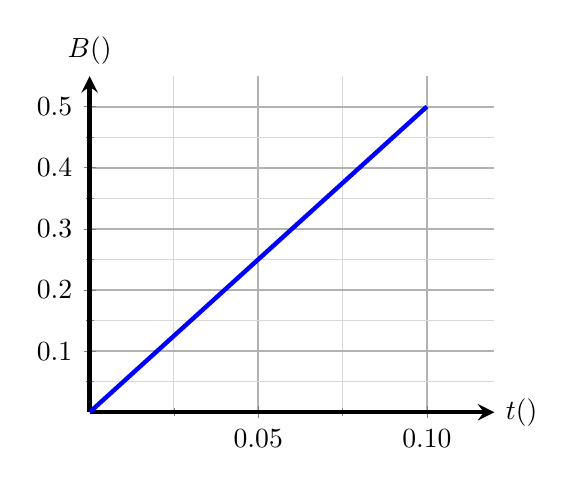
\begin{tikzpicture}  
			\begin{axis}[  ultra thick,scale=0.75,
				xmin=0,  
				xmax=0.12,  
				xtick={0,0.05,...,0.10},
				ytick={0,0.1,...,0.5},
				minor x tick num=1,
				minor y tick num=1,
				ymin=0,  
				ymax=0.55, 
				samples=300,
				xticklabel style={/pgf/number format/.cd, fixed,
					fixed zerofill, precision=2},
				axis lines=center, 
				grid style={step=1, line width =0.4pt, color=gray!30!white},
				grid=both, %giới hạn ô lưới
				major grid style={line width=0.8pt,gray!60!white},
				xlabel=$\xsi{t}{\left(\si{\second}\right)}$, 		ylabel=$\xsi{B}{\left(\si{\tesla}\right)}$,
				every axis y label/.style={at=(current axis.above origin),anchor=south},  
				every axis x label/.style={at=(current axis.right of origin),anchor=west},]
				\addplot [ultra thick, blue, smooth, domain=0:0.1] {5*x};  
			\end{axis}  
		\end{tikzpicture}
	\end{center}
	
	\choice
	{\True $\SI{2.5}{\volt}$}
	{$\SI{-5}{\volt}$}
	{$\SI{-2.5}{\volt}$}
	{$\SI{5}{\volt}$}
	\loigiai{
		$$
		\begin{aligned}
			&\text { Độ lớn suất điện động cảm ứng sinh ra trong vòng dây là: }\\
			&|e|=\left|\frac{\Delta \Phi}{\Delta t}\right|=\left|\frac{S\Delta B}{\Delta t}\right|=\left|\frac{0,5 \cdot 0,5}{0,1}\right|=\SI{2.5}{\volt}
		\end{aligned}
		$$
	}
\end{ex}
% ===================================================================
\begin{ex}
	Một vật nhỏ khối lượng $\SI{2}{\kilogram}$, có chuyển động trượt với vận tốc $\SI{4}{\meter/\second}$ về phía trái trên một mặt phẳng ngang. Vào một thời điểm nào đó, người ta tác dụng vào vật một lực $\vec{F}$ nằm ngang hướng về bên phải. Sau đó một khoảng thời gian, vận tốc của vật hướng sang bên phải, độ lớn $\SI{4}{\meter/\second}$. Công của lực $F$ trong khoảng thời gian nói trên là
	\choice
	{\True$\SI{0}{\joule}$}
	{$\SI{8}{\joule}$}
	{$\SI{16}{\joule}$}
	{$\SI{32}{\joule}$}
	\loigiai{
	Áp dụng định lý động năng:
	$$A_{F}=\dfrac{1}{2}m\left(v^2_2-v^2_1\right)=\SI{0}{\joule}.$$
	}
\end{ex}
% ===================================================================
\begin{ex}
	Hình bên dưới là mặt đồng hồ của máy bay thế chiến II phát sáng trong bóng tối, vì chúng được sơn bằng sơn phát quang pha radium (có chu kì bán rã 1602 năm). Mặc dù mặt đồng hồ sơn radium có thể nhìn thấy dễ dàng cả ngày lẫn đêm, nhưng chúng phát ra radon, một loại khí phóng xạ nguy hiểm và không thể cảm nhận trực tiếp. 
	\begin{center}
		\includegraphics[width=0.4\linewidth]{../figs/BThatnhan-4}\\
		\textit{Mặt đồng hồ trong máy bay được sơn bằng sơn phát quang có pha radium.}
	\end{center}
	Nếu độ phóng xạ ban đầu của radium khi mới được sơn là $\SI{E5}{\becquerel}$ thì độ phóng xạ còn lại sau 57 năm kể từ khi sản xuất là
	\choice
	{$\SI{96504.5}{\becquerel}$}
	{$\SI{2436.1}{\becquerel}$}
	{\True $\SI{97563.9}{\becquerel}$}
	{$\SI{3495.5}{\becquerel}$}
	\loigiai{
		Độ phóng xạ còn lại:
		$$H=H_0\cdot 2^{-\dfrac{t}{T}}=\left(\SI{E5}{\becquerel}\right)\cdot 2^{-\dfrac{57}{1602}}\approx\SI{97563.9}{\becquerel}.$$
	}
\end{ex}
% ===================================================================
\begin{ex}
	Chọn đáp án \textbf{đúng}.\\
	Dựa vào đồ thị biểu diễn năng lượng liên kết riêng của các hạt nhân theo số khối, sự sắp xếp theo độ bền vững tăng dần của 3 hạt nhân vàng $\left(\ce{Au}\right)$, chlorine $\left(\ce{Cl}\right)$ và sắt $\left(\ce{Fe}\right)$ là
	\begin{center}
		\includegraphics[width=0.7\linewidth]{../figs/VN12-Y24-PH-SYL-027P-3}
	\end{center}
	\choice
	{$\ce{Cl}$, $\ce{Au}$, $\ce{Fe}$}
	{$\ce{Fe}$, $\ce{Au}$, $\ce{Cl}$, }
	{\True $\ce{Au}$, $\ce{Cl}$, $\ce{Fe}$}
	{$\ce{Cl}$, $\ce{Fe}$, $\ce{Au}$}
	\loigiai{}
\end{ex}
% ===================================================================
\begin{ex}
	Trên mặt phẳng nằm ngang không ma sát có ba hòn bi hoàn toàn giống nhau cùng nằm trên một đường thẳng. Hai hòn bi 2 và 3 đứng yên, tiếp xúc với nhau, hòn bi 1 tới va chạm vào hòn bi 2 với vận tốc $v_0$. 
	\begin{center}
		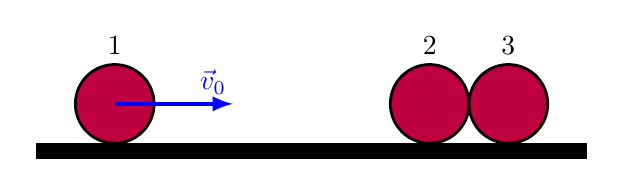
\begin{tikzpicture}
			\filldraw[line width=1pt, draw=black, fill=purple] (0,0.5) circle(0.5);
			\filldraw[line width=1pt, draw=black, fill=purple] (4,0.5) circle(0.5);
			\filldraw[line width=1pt, draw=black, fill=purple] (5,0.5) circle(0.5);
			\draw[line width=6pt] (-1,-0.1)--(6,-0.1);
			\draw[-latex, blue, line width=1.5pt] (0,0.5)--(1.5,0.5);
			\node[above, blue] at (1.25,0.5) {$\vec{v}_0$};
			\node[above] at (0,1) {1};
			\node[above] at (4,1) {2};
			\node[above] at (5,1) {3};
		\end{tikzpicture}
	\end{center}
	Bỏ qua sự mất mát động năng do va chạm. Tốc độ 3 hòn bi sau va chạm sẽ là
	\choice
	{$v_1=v_2=v_3=\dfrac{v_0}{\sqrt{3}}$}
	{$v_1=0$, $v_2=v_3=\dfrac{v_0}{\sqrt{3}}$}
	{$v_3=0$, $v_1=v_2=\dfrac{v_0}{\sqrt{3}}$}
	{\True $v_1=v_2=0$, $v_3=v_0$}
	\loigiai{
		Công thức va chạm đàn hồi:
		$$v'_1=\dfrac{\left(m_1-m_2\right)v_1+2m_2v_2}{m_1+m_2}$$
		$$v'_2=\dfrac{\left(m_2-m_1\right)v_2+2m_1v_1}{m_1+m_2}$$
		Do đó, sau quá trình va chạm của quả cầu 1 và 2 thì $v_2'=v_0; v'_1=0$.\\
		Tương tự, sau va chạm của quả cầu 2 và 3 thì $v'_3=v_0; v''_2=0$.
	}
\end{ex}
% ===================================================================
\begin{ex}
	Một sóng cơ hình sin truyền dọc theo chiều dương của trục $Ox$, đường vẽ liền nét là hình dạng của sóng tại một thời điểm, đường đứt nét là hình dạng của sóng đó sau thời điểm trên $\SI{0.2}{\second}$.
	\begin{center}
		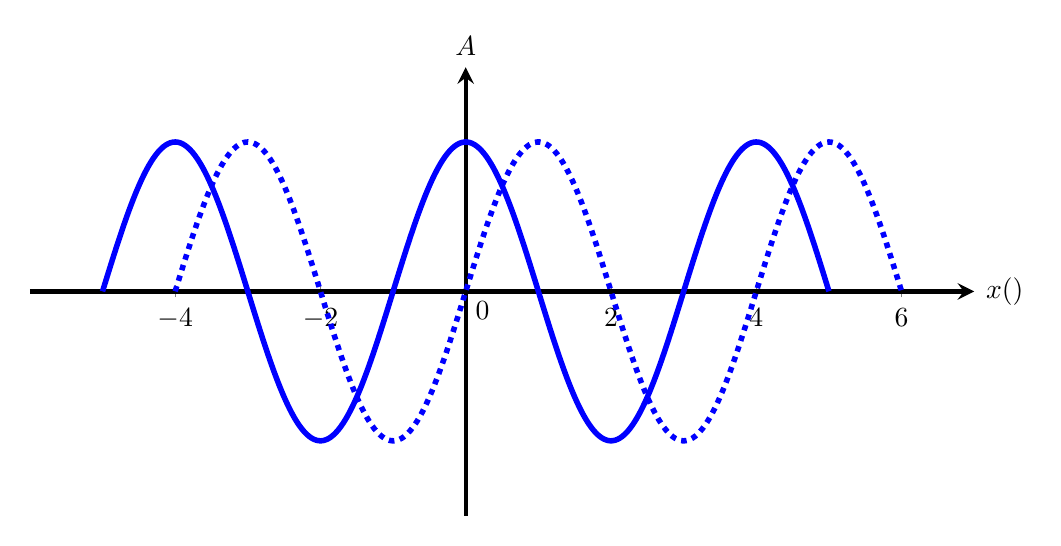
\begin{tikzpicture}  
			\begin{axis}[  ultra thick,xscale=1.75,
				xmin=-6,  
				xmax=7,  
				xtick={-4,-2,...,6},
				minor x tick num=0,
				ymin=-3,  
				ymax=3, 
				samples=300,
				yticklabels=\empty,
				ytick=\empty,
				axis lines=center,
				xlabel=$\xsi{x}{\left(\si{\meter}\right)}$, 		ylabel=$A$,
				ylabel style={above}, 
				every axis x label/.style={at=(current axis.right of origin),anchor=west},  ]
				\addplot [line width=2pt, blue, smooth, domain=-5:5] {2*cos(deg(pi*x/2))};  
				\addplot [line width=2pt, blue,dotted, smooth, domain=-4:6] {2*cos(deg(pi*x/2-pi/2))};  
				\coordinate (O) at (axis cs: 0,0);
			\end{axis}  
			\node[below right] at (O) {0};
		\end{tikzpicture}
	\end{center} 
	Tốc độ truyền sóng là
	\choice
	{$\xsi{20\cdot\left(n+\dfrac{3}{4}\right)}{\centi\meter/\second}$ với $n\in\mathbb{N}$}
	{\True $\xsi{20\cdot\left(n+\dfrac{1}{4}\right)}{\centi\meter/\second}$ với $n\in\mathbb{N}$}
	{$\xsi{20\cdot\left(n+\dfrac{1}{2}\right)}{\centi\meter/\second}$ với $n\in\mathbb{N}$}
	{$\xsi{20n}{\centi\meter/\second}$ với $n\in\mathbb{N}$}
	\loigiai{
		Tốc độ truyền sóng:
		$$v=\dfrac{s}{t}=\dfrac{\lambda\left(\dfrac{1}{4}+n\right)}{\SI{0.2}{\second}}=\dfrac{\left(\SI{4}{\centi\meter}\right)\cdot\left(\dfrac{1}{4}+n\right)}{\SI{0.2}{\second}}=\xsi{20\cdot\left(n+\dfrac{1}{4}\right)}{\centi\meter/\second}.$$
	}
\end{ex}
% ===================================================================
\begin{ex}
Cho mạch điện có sơ đồ như hình vẽ.\\
Nguồn điện có suất điện động $\calE=\SI{12}{\volt}$, điện trở trong không đáng kể. Tụ điện có điện dung $\SI{2}{\micro\farad}$, các điện trở có giá trị thỏa $R_1:R_2:R_3:R_4=1:2:6:3$. Điện tích của bản cực a là	
\begin{center}
\begin{circuitikz}%[european]
			\coordinate (A) at (-3,0);
			\coordinate (B) at ($(A)+(30:3)$);
			\coordinate (C) at ($(B)+(-30:3)$);
			\coordinate (R1) at ($(A)!0.5!(B)$);
			\coordinate (D) at ($(A)+(-30:3)$);
			\draw (A) to [R=$R_1$] (B)
			(B) to [R=$R_2$] (C)
			(A) to [R=$R_3$] (D)
			(D) to [R=$R_4$] (C)
			(B) to [C=$C$] (D)
			(A)--++(0,-3) to[battery2, l=$\calE$]++(5.196,0)--++(0,3)
			;
			\node[above left] at($(B)-(0,1.4)$) {a};
			\node[below left] at($(B)-(0,1.6)$) {b};
\end{circuitikz}
\end{center}
	\choice
	{$\SI{-8E-6}{\coulomb}$}
	{$\SI{-4E-6}{\coulomb}$}
	{\True $\SI{8E-6}{\coulomb}$}
	{$\SI{4E-6}{\coulomb}$}
	\loigiai{
	
	}
\end{ex}




% ===================================================================
\begin{ex}
	\immini{Hình vẽ là đồ thị biểu diễn sự thay đổi áp suất $p$ theo nhiệt độ tuyệt đối $T$ của một khối khí lí tưởng. Khối khí này bắt đầu biến đổi từ trạng thái A, sang trạng thái B, rồi chuyển sang trạng thái C với khối lượng riêng ở các trạng thái tương ứng là $\rho_{\mathrm{A}}$, $\rho_{\mathrm{B}}$, $\rho_{\mathrm{C}}$. So sánh đúng là}
	{
	\begin{tikzpicture}  
		\begin{axis}[  ultra thick, scale=0.5,
			xmin=0,  
			xmax=7,  
			ymin=0,  
			ymax=7.25, 
			samples=300,
			yticklabels=\empty,
			xticklabels=\empty,
			xtick=\empty,
			ytick=\empty,
			xlabel=$\xsi{T}{\left(\si{\kelvin}\right)}$, 		ylabel=$p$,
			axis lines=center, 
			every axis y label/.style={at=(current axis.above origin),anchor=south},  
			every axis x label/.style={at=(current axis.right of origin),anchor=west},  ]
			\coordinate (A) at (axis cs: 1,0.5);
			\coordinate (B) at (axis cs: 6,3);
			\coordinate (C) at (axis cs: 6,6);
			\draw[dashed, line width=1pt] (axis cs: 0,0)--(A);
			\draw[
			decoration={markings, mark=at position 0.5 with {\arrow{stealth}}},
			postaction={decorate}, line width=2pt, blue
			] (A)--(B);
			\draw[
			decoration={markings, mark=at position 0.5 with {\arrow{stealth}}},
			postaction={decorate}, line width=2pt, blue
			] (B)--(C);
			\coordinate (O) at (axis cs: 0,0);
			\fill   (A) circle[radius=2pt]  node [above] {A};
			\fill   (B) circle[radius=2pt]  node [below] {B};
			\fill   (C) circle[radius=2pt]  node [above] {C};
		\end{axis}  
		\node[below left] at (O) {O};
	\end{tikzpicture}
	}
	\choice
	{$\rho_{\mathrm{A}}>\rho_{\mathrm{B}}>\rho_{\mathrm{C}}$}
	{\True $\rho_{\mathrm{A}}=\rho_{\mathrm{B}}<\rho_{\mathrm{C}}$}
	{{$\rho_{\mathrm{A}}<\rho_{\mathrm{B}}=\rho_{\mathrm{C}}$}}
	{{$\rho_{\mathrm{A}}=\rho_{\mathrm{B}}=\rho_{\mathrm{C}}$}}
	\loigiai{
		$\rho=\dfrac{m}{V}\Rightarrow V$ càng bé thì $\rho$ càng lớn.\\
		AB là quá trình đẳng tích $\Rightarrow V_{\mathrm{A}}=V_{\mathrm{B}}\Rightarrow \rho_{\mathrm{A}}=\rho_{\mathrm{B}}$\\
		BC là quá trình đẳng nhiệt $\Rightarrow pV=const$ mà $p_{\mathrm{B}}<p_{\mathrm{C}}\Rightarrow V_{\mathrm{B}}>V_{\mathrm{C}}\Rightarrow \rho_{\mathrm{B}}<\rho_{\mathrm{C}}$.
	}
\end{ex}

% ===================================================================
\begin{ex}
	Một điện áp xoay chiều $u=U_0\cos\left(\omega t+\varphi_u\right)$ có đồ thị điện áp - thời gian như Hình \ref{fig: 23P-1}a. Lần lượt sử dụng điện áp xoay chiều này đặt vào các đoạn mạch A, B, C có chứa các linh kiện điện tử, ta thu được đồ thị cường độ dòng điện - thời gian như Hình \ref{fig: 23P-1}b
	\begin{center}
		\begin{tabular}{M{8.5cm}M{8.5cm}}
			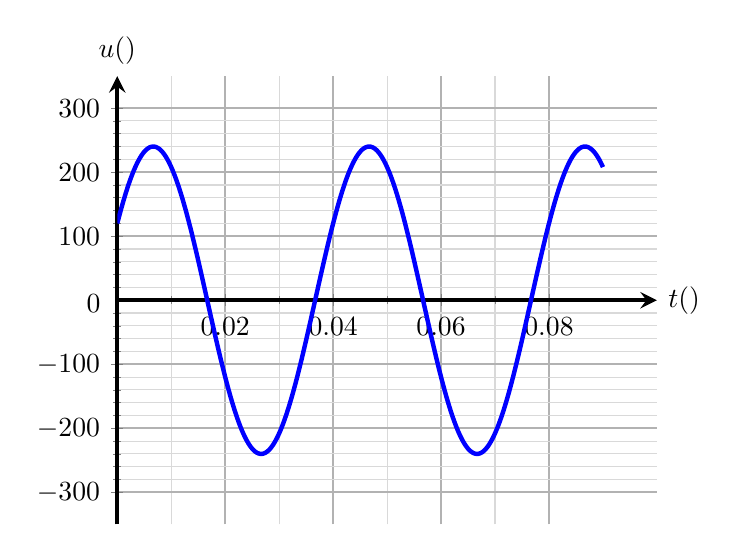
\begin{tikzpicture}  
				\begin{axis}[  ultra thick,
					xmin=0,  
					xmax=0.1,  
					xtick={0,0.02,...,0.08},
					ytick={-300,-200,...,300},
					minor x tick num=1,
					minor y tick num=4,
					ymin=-350,  
					ymax=350, 
					samples=300,
					xticklabel style={/pgf/number format/.cd, fixed,
						fixed zerofill, precision=2}, %số chữ số thập phân
					axis lines=center, 
					grid style={step=1, line width =0.4pt, color=gray!30!white},
					grid=both, %giới hạn ô lưới
					major grid style={line width=0.8pt,gray!60!white},
					xlabel=$\xsi{t}{\left(\si{\second}\right)}$, 		ylabel=$\xsi{u}{\left(\si{\volt}\right)}$,
					every axis y label/.style={at=(current axis.above origin),anchor=south},  
					every axis x label/.style={at=(current axis.right of origin),anchor=west},  ]
					\addplot [ultra thick, blue, smooth, domain=0:0.09] {240*cos(deg(50*pi*x-pi/3))};   
				\end{axis} 
				\node at (-0.3,2.8) {0}; 
			\end{tikzpicture}
			& 
			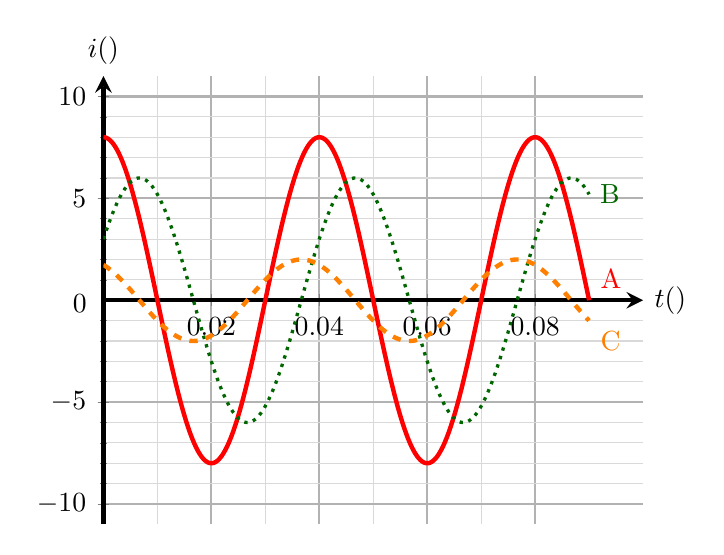
\begin{tikzpicture}  
				\begin{axis}[  ultra thick,
					xmin=0,  
					xmax=0.1,  
					xtick={0,0.02,...,0.08},
					ytick={-10,-5,...,10},
					minor x tick num=1,
					minor y tick num=4,
					ymin=-11,  
					ymax=11, 
					samples=300,
					xticklabel style={/pgf/number format/.cd, fixed,
						fixed zerofill, precision=2}, %số chữ số thập phân
					axis lines=center, 
					grid style={step=1, line width =0.4pt, color=gray!30!white},
					grid=both, %giới hạn ô lưới
					major grid style={line width=0.8pt,gray!60!white},
					xlabel=$\xsi{t}{\left(\si{\second}\right)}$, 		ylabel=$\xsi{i}{\left(\si{\ampere}\right)}$,
					every axis y label/.style={at=(current axis.above origin),anchor=south},  
					every axis x label/.style={at=(current axis.right of origin),anchor=west},  ]
					\addplot [ultra thick, red, smooth, domain=0:0.09] {8*cos(deg(50*pi*x))} node[red, above right] {A};   
					\addplot [very thick, green!40!black, smooth,dotted, domain=0:0.09] {6*cos(deg(50*pi*x-pi/3))} node[green!40!black, right] {B}; 
					\addplot [ultra thick, orange, smooth,dashed, domain=0:0.09] {2*cos(deg(50*pi*x+pi/6))} node[orange, below right] {C}; 
				\end{axis} 
				\node at (-0.3,2.8) {0}; 
			\end{tikzpicture}\\
			a) & b)
		\end{tabular}
		\captionof{figure}{}
		\label{fig: 23P-1}
	\end{center}
	Chỉ ra phát biểu \textbf{sai}.
	\choice
	{Tần số của điện áp xoay chiều và tần số của cường độ dòng điện trong ba đoạn mạch (A), (B), (C) là $\SI{25}{\hertz}$}
	{\True Pha ban đầu của cường độ dòng điện trong ba đoạn mạch (A), (B), (C) lần lượt là $\SI{0}{\radian}$, $\xsi{\dfrac{\pi}{3}}{\radian}$, $\xsi{\dfrac{\pi}{6}}{\radian}$}
	{Đoạn mạch (B) chỉ chứa điện trở thuần và có giá trị $R=\SI{40}{\ohm}$}
	{Cường độ dòng điện trong mạch điện (C) vuông pha với điện áp xoay chiều}
	\loigiai{
		Tần số của điện áp xoay chiều và tần số của cường độ dòng điện trong ba đoạn mạch (A), (B), (C) là:
		$$
		f=\dfrac{1}{T}=\frac{1}{0,04}=\SI{25}{\hertz}.
		$$
		Pha ban đầu của điện áp xoay chiều và cường độ dòng điện trong ba đoạn mạch (A), (B), (C) lần lượt là: $\varphi_{\mathrm{u}}=\xsi{-\dfrac{\pi}{3}}{\radian}$, $\varphi_{i(A)}=\SI{0}{\radian}$, $\varphi_{i(B)}=\xsi{-\dfrac{\pi}{3}}{\radian}$, $\varphi_{i(c)}=\xsi{\dfrac{\pi}{6}}{\radian}$.\\
		Cường độ dòng điện và điện áp xoay chiều trong đoạn mạch (B) dao động cùng pha với nhau nên mạch chỉ chứa điện trở thuần và có giá trị:
		$$
		R=\frac{U_0}{I_0}=\frac{240}{6}=\SI{40}{\ohm}.
		$$	
	}
\end{ex}

% ===================================================================
\begin{ex}
	Bắn hạt neutron có động năng $\SI{2}{\mega\electronvolt}$ vào hạt nhân $\ce{^6_3Li}$   đứng yên gây ra phản ứng $\ce{^1_0n}+\ce{^6_3Li}\longrightarrow\ce{X}+\alpha$. Hạt $\alpha$ và hạt nhân $\ce{X}$ bay ra theo các hướng hợp với hướng tới của neutron những góc tương ứng bằng $\theta=\SI{15}{\degree}$ và $\varphi=\SI{30}{\degree}$. Lấy tỉ số giữa khối lượng của các hạt nhân bằng tỉ số giữa các số khối của chúng. Bỏ qua bức xạ gamma. Năng lượng của phản ứng hạt nhân trên là
	\choice
	{Tỏa $\SI{1.52}{\mega\electronvolt}$}
	{Thu $\SI{1.52}{\mega\electronvolt}$}
	{\True Thu $\SI{1.66}{\mega\electronvolt}$}
	{Tỏa $\SI{1.66}{\mega\electronvolt}$}
	\loigiai{
		Áp dụng định luật bảo toàn động lượng:
		$$\vec{p}_{\ce{n}}=\vec{p}_{\ce{X}}+p_{\ce{\alpha}}$$
		\begin{center}
			\includegraphics[width=0.4\linewidth]{../figs/VN12-Y24-PH-SYL-029P-1}
		\end{center}
		Áp dụng định lý hàm sin trong tam giác động lượng:
		$$\dfrac{p_{\ce{n}}}{\sin\SI{135}{\degree}}=\dfrac{p_{\alpha}}{\sin\SI{30}{\degree}}\Rightarrow \dfrac{\sqrt{2m_{\ce{n}}K_{\ce{n}}}}{\sin\SI{135}{\degree}}=\dfrac{\sqrt{2m_{\alpha}K_{\alpha}}}{\sin\SI{30}{\degree}}\Rightarrow K_{\alpha}=\SI{0.25}{\mega\electronvolt}.$$
		Tương tự: $K_{\ce{X}}\approx\SI{0.089}{\mega\electronvolt}$.\\
		Năng lượng phản ứng:
		$$E=K_{\alpha}+K_{\ce{X}}-K_{n}=\SI{-1.66}{\mega\electronvolt}.$$
	}
\end{ex}
% ===================================================================
\begin{ex}
	\immini{
	Trong hình bên, đoạn dây dẫn thẳng đứng có dòng điện $I$ đi qua được đặt song song với một khung dây nhỏ ở trong cùng mặt phẳng. Để cho hợp lực tác dụng lên khung có chiều hướng sang phải thì khung phải di chuyển theo hướng
	\choice
	{đi lên}
	{đi xuống}
	{sang phải}
	{\True sang trái}
	}
	{
	\begin{tikzpicture}
		\draw[decoration={markings, mark=at position 0.5 with {\arrow{stealth}}},
		postaction={decorate}, line width=2pt, blue] (0,0)--(0,3);
		\draw[line width=1.5pt] (1,0.5)--(1,2.5)--(2,2.5)--(2,0.5)--(1,0.5);
		\node[left] at(0,1.5) {$I$};
	\end{tikzpicture}
	}
	\loigiai{}
\end{ex}
% ===================================================================
\begin{ex}
	\immini{Một bình chứa khí được chia làm 2 ngăn A và B bởi piston cách nhiệt. Ban đầu, piston bị chốt lại để thể tích khí ở ngăn A gấp 1,5 lần thể tích khí ở ngăn B. Lúc này, khí ở ngăn A có nhiệt độ $\SI{177}{\celsius}$ và áp suất $\SI{1.5}{atm}$,  khí ở ngăn B có nhiệt độ $\SI{27}{\celsius}$ và áp suất $\SI{1.2}{atm}$. }
	{\includegraphics[width=0.5\linewidth]{{../figs/DGNL-2}}}
	Người ta tháo chốt để piston chuyển động tự do trong bình. Do thành bình dẫn nhiệt chậm nên khí A và B cuối cùng đạt đến nhiệt độ phòng là $\SI{27}{\celsius}$. Khi piston dừng lại, áp suất khí trong mỗi bình là
	\choice
	{$\SI{1.12}{atm}$}
	{$\SI{1.05}{atm}$}
	{\True $\SI{1.08}{atm}$}
	{$\SI{0.90}{atm}$}
	\loigiai{
		\begin{center}
			\begin{tabular}{|M{4cm}|M{4cm}|M{4cm}|M{4cm}|}
				\hline
				\thead{Trạng thái}& $p$ & $V$ & $T$\\
				\hline
				Phần A ban đầu & $\SI{1.5}{atm}$& $3V$ &$\SI{450}{\kelvin}$\\
				\hline
				Phần B ban đầu & $\SI{1.2}{atm}$ & $2V$ & $\SI{300}{\kelvin}$\\
				\hline
				Phần A lúc sau & $p'$ & $V'_{\mathrm{A}}$ & $\SI{300}{\kelvin}$\\
				\hline
				Phần B lúc sau & $p'$ & $V'_{\mathrm{B}}$& $\SI{300}{\kelvin}$\\
				\hline
			\end{tabular}
		\end{center}
		$$\dfrac{pV}{T}=const\Rightarrow \begin{cases}
			\frac{1,5\cdot3V}{450}=\frac{p'\cdot V'_{\mathrm{A}}}{300}\\
			\frac{1,2\cdot2V}{300}=\frac{p'\cdot V'_{\mathrm{B}}}{300}
		\end{cases}\Rightarrow\begin{cases}
			V'_{\mathrm{A}}=\frac{3V}{p'}\\
			V'_{\mathrm{B}}=\frac{2,4V}{p'}
		\end{cases}$$
		Mà:
		$$V'_{\mathrm{A}}+V'_{\mathrm{B}}=3V+2V\Leftrightarrow\dfrac{3}{p'}+\dfrac{2,4}{p'}=3+2\Rightarrow p'=\SI{1.08}{atm}.$$
	}
\end{ex}
% ===================================================================
\begin{ex}
	Trong khảo cổ học để đánh giá tuổi của các vật liệu hữu cơ như gỗ và da, người ta thường sử dụng kỹ thuật xác định tuổi bằng carbon phóng xạ. Cơ sở của kĩ thuật này là mật độ  nguyên tử $\ce{^{14}C}$ trong khí quyển gần như không đổi và có giá trị bằng $1,3$ nguyên tử $\ce{^{14}C}$ trong mỗi $10^{12}$ nguyên tử carbon bao gồm tất cả các đồng vị. Tuy nhiên, khi một cơ thể sống chết đi, $\ce{^{14}C}$ không còn được cung cấp nữa và bắt đầu giảm đi phóng xạ $\beta$ với thời gian bán rã $\SI{5730}{\text{năm}}$:
	$$\ce{^{14}_6C}\longrightarrow \ce{^{14}_7N}+e^{-}+\overline{\nu}_e$$
	Giả sử có $\SI{50}{\gram}$ carbon từ một mảnh gỗ tìm được trong một ngôi mộ tiền sử. Biết khối lượng nguyên tử trung bình của carbon là $\SI{2e-26}{\kilogram}$. Người ta không thể đếm trực tiếp số nguyên tử $\ce{^{14}C}$ được nhưng có thể đếm được tổng số $935$ electron phát xạ từ mảnh gỗ trên trong 10 phút. Tuổi của ngôi mộ là
	\choice
	{19359 năm}
	{\True 17190 năm}
	{13223 năm}
	{15021 năm}
	\loigiai{
		Số nguyên tử $\ce{^{14}C}$ ban đầu trong mảnh gỗ:
		$$N_0=\dfrac{m}{m_0}\cdot\dfrac{1,3}{10^{12}}=\SI{3.25E12}{}.$$
		Độ phóng xạ của mẫu gỗ ở thời điểm phát hiện:
		$$H=\dfrac{\Delta N}{\Delta t}=\lambda N_0e^{-\lambda T}$$
		Tuổi của mẫu vật:
		$$\begin{aligned}
			&t=-\dfrac{1}{\lambda}\cdot\ln\left(\dfrac{1}{\lambda N_0}\cdot\dfrac{\Delta N}{\Delta t}\right)=-\dfrac{T}{\ln2}\cdot\ln\left(\dfrac{T}{N_0\ln 2}\cdot\dfrac{\Delta N}{\Delta t}\right)\\
			\Rightarrow &t=-\dfrac{\left(\SI{5730}{\text{năm}}\right)}{\ln2}\cdot\ln\left(\dfrac{5730\cdot365\cdot24\cdot\SI{60}{\minute}}{\SI{3.25E12}{}\cdot\ln2}\cdot\dfrac{935}{\SI{10}{\minute}}\right)\approx\SI{17190}{\text{năm}}.
		\end{aligned}
		$$}
\end{ex}
\Closesolutionfile{ans}
\section{Câu trắc nghiệm đúng/sai} 
\textit{Thí sinh trả lời từ câu 1 đến câu 4. Trong mỗi ý \textbf{a)}, \textbf{b)}, \textbf{c)}, \textbf{d)} ở mỗi câu, thí sinh chọn đúng hoặc sai}
\setcounter{ex}{0}
\Opensolutionfile{ans}[ans/G11-4-TF]
% ===================================================================
\begin{ex}
	Cho các phát biểu dưới đây. Phát biểu nào là phát biểu đúng, phát biểu nào sai?
	\choiceTF[t]
	{\True Dao động điều hòa là dao động có li độ biến thiên theo thời gian theo qui luật hàm sin hoặc cosin}
	{\True Chu kì là khoảng thời gian ngắn nhất mà trạng thái dao động của vật được lặp lại như cũ}
	{Một vật dao động tuần hoàn thì chắc chắn dao động điều hòa}
	{Cơ năng của vật dao động điều hòa biến thiên tuần hoàn theo thời gian}
	\loigiai{}
\end{ex}
% ===================================================================
\begin{ex}
	Một vật nhỏ có khối lượng $\SI{100}{\gram}$ dao động điều hòa với phương trình $x=\xsi{4\cos\left(5\pi t+\dfrac{\pi}{3}\right)}{\centi\meter}$, $t$ được tính bằng giây. Lấy $\pi^2\approx10$.
	\choiceTF[t]
	{\True Chu kì dao động của vật là $\SI{0.4}{\second}$}
	{Tốc độ cực đại của vật là  $\xsi{20\sqrt{10}}{\meter/\second}$}
	{\True Năng lượng dao động của vật là $\SI{0.02}{\joule}$}
	{Trong khoảng thời gian $t =\SI{1.2}{\second}$, vật đi được quãng đường $\SI{12}{\centi\meter}$}
	\loigiai{}
\end{ex}
% ===================================================================
\begin{ex}
	Vật nhỏ dao động điều hòa trên trục $Ox$, vật đi từ biên này đến biên kia mất $\SI{0.157}{\second}$; khoảng cách giữa hai biên là $\SI{10}{\centi\meter}$. Lấy $\pi=3,14$.
	\choiceTF[t]
	{Chu kì dao động của vật là $\SI{0.157}{\second}$}
	{\True Vật thực hiện được 10 dao động trong $\SI{3.14}{\second}$}
	{\True Thời gian ngắn nhất vật đi từ vị trí $x =\SI{5}{\centi\meter}$ đến $x =\SI{-2.5}{\centi\meter}$ là $\SI{0.105}{\second}$}
	{\True Tốc độ của vật khi qua vị trí cân bằng là $\SI{1}{\meter/\second}$}
	\loigiai{}
\end{ex}
% ===================================================================
\begin{ex}
	Một vật dao động điều hòa có phương trình $x=\xsi{4\cos\left(2\pi t-\dfrac{\pi}{2}\right)}{\centi\meter}$. 
	\choiceTF[t]
	{Vật chuyển động trên quỹ đạo dài $\SI{4}{\centi\meter}$}
	{\True Phương trình vận tốc của vật có dạng là $v=\xsi{-8\pi\sin\left(2\pi t-\dfrac{\pi}{2}\right)}{\centi\meter/\second}$}
	{\True Tại vị trí $x=\pm\dfrac{A\sqrt{3}}{2}$  thì động năng bằng một phần ba thế năng}
	{\True Đồ thị tọa độ - thời gian của vật là hình dưới đây\\
		\includegraphics[width=0.4\linewidth]{../figs/D11-004-3}
	}
	\loigiai{}
\end{ex}

\Closesolutionfile{ans}
\section{Câu trắc nghiệm trả lời ngắn} 
\textit{Ứng viên trả lời từ câu 1 đến câu 5}
\setcounter{ex}{0}
\Opensolutionfile{ans}[ans/DGNL-TL]
% ===============================================================
\begin{ex}
	Ở giai đoạn cuối của quá trình tiến hoá sao, một ngôi sao có khối lượng gấp đôi khối lượng Mặt Trời sẽ suy sụp hấp dẫn ở nhân, tổng hợp proton và electron của nó lại để tạo thành sao neutron. Do đó, ngôi sao lúc này có thể được coi là một hạt nhân nguyên tử khổng lồ. Nếu một ngôi sao có khối lượng $2\times\SI{1.99E30}{\kilogram}$ suy sụp thành các neutron ($m_n=\SI{1.67E-27}{\kilogram}$)  thì bán kính sao neutron lúc này là bao nhiêu? Giả sử bán kính $r=r_0A^{\frac{1}{3}}$, với $r_0=\SI{1.2}{\femto\meter}$. \textit{(Kết quả tính theo đơn vị kilomet và làm tròn đến phần nguyên)}.
	\shortans{16}
	\loigiai{
		Số neutron trong ngôi sao:
		$$A=\dfrac{m}{m_n}$$
		Bán kính sao:
		$$r=r_0A^{\frac{1}{3}}=r_0\left(\dfrac{m}{m_n}\right)^{\frac{1}{3}}=\left(\SI{1.2E-15}{\meter}\right)\cdot\left[\dfrac{2\times\SI{1.99E30}{\kilogram}}{\SI{1.67E-27}{\kilogram}}\right]^{\frac{1}{3}}
		\approx\SI{16028.9}{\meter}=\SI{16.03}{\kilo\meter}.$$}
\end{ex}
% =============================================================
\begin{ex}
	Đặt vào hai đầu cuộn sơ cấp của máy biến áp lí tưởng (bỏ qua hao phí) một điện áp xoay chiều có giá trị hiệu dụng không đổi thì điện áp hiệu dụng giữa hai đầu cuộn thứ cấp để hở là $\SI{100}{\volt}$. Ở cuộn thứ cấp, nếu giảm bớt $n$ vòng dây thì điện áp đó là $2U$. Nếu tăng thêm $1,5n$ vòng dây ở cuộn thứ cấp thì điện áp hiệu dụng giữa hai đầu để hở của cuộn này bằng bao nhiêu volt?
	\shortans{$150$}
	\loigiai{
		Ta có: $\dfrac{U_1}{U_2}=\dfrac{N_1}{N_2}$
		\begin{equation}
			\label{eq: 1}\\
			\Rightarrow U_2=\dfrac{N_2U_1}{N_1}=\SI{100}{\volt}	
		\end{equation}
		\begin{equation}
			\label{eq: 2}\\
			\dfrac{N_1}{N_2-n}=\dfrac{U_1}{U}
		\end{equation}
		\begin{equation}
			\label{eq: 3}\\
			\dfrac{N_1}{N_2+n}=\dfrac{U_1}{2U}
		\end{equation}
		Từ \eqref{eq: 2} và \eqref{eq: 3}
		\begin{equation}
			\label{eq: 4}\\
			\Rightarrow N_2=3n
		\end{equation}
		\begin{equation}
			\label{eq: 5}\\
			\dfrac{N_1}{N_2+1,5n}=\dfrac{U_1}{U_3}\Rightarrow U_3=\dfrac{U_1}{N_1}\left(N_2+1,5n\right)
		\end{equation}
		Từ \eqref{eq: 1}, \eqref{eq: 4}, \eqref{eq: 5} $\Rightarrow U_3=\SI{150}{\volt}$.
	}
\end{ex}
% ===============================================================
\begin{ex}
	Một lượng khí lí tưởng đơn nguyên tử chuyển từ trạng thái (1) sang trạng thái (2) bằng hai cách:
	\begin{itemize}
		\item Cách 1: $(1)\rightarrow (3)\rightarrow (2)$.
		\item Cách 2: $(1)\rightarrow(4)\rightarrow (2)$.
	\end{itemize}
	\begin{center}
		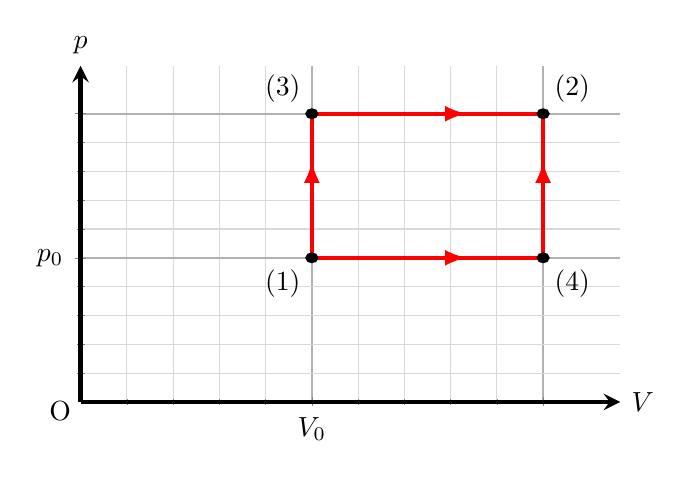
\begin{tikzpicture}  
			\begin{axis}[  ultra thick, yscale=0.75,
				xmin=0,  
				xmax=7,  
				ytick={0,3,6},
				xtick={0,3,6},
				ymin=0,  
				ymax=7, 
				samples=300,
				yticklabels={,$p_0$,},
				xticklabels={,$V_0$,},
				axis lines=center, 
				xlabel=$V$, 
				ylabel=$p$, 
				every axis y label/.style={at=(current axis.above origin),anchor=south},  
				every axis x label/.style={at=(current axis.right of origin),anchor=west},
				minor x tick num=4,
				minor y tick num=4,
				grid style={step=1, line width =0.4pt, color=gray!30!white},
				grid=both,
				major grid style={line width=0.8pt,gray!60!white},
				]
				\draw[ultra thick, red] (axis cs: 3, 3) -- (axis cs:6, 3);
				\draw[ultra thick,-latex, red] (axis cs: 3, 3) -- (axis cs: 5, 3);
				\draw[ultra thick, red] (axis cs: 3, 6) -- (axis cs:6, 6);
				\draw[ultra thick,-latex, red] (axis cs: 3, 6) -- (axis cs: 5, 6);
				\draw[ultra thick, red] (axis cs: 3, 3) -- (axis cs:3, 6);
				\draw[ultra thick,-latex, red] (axis cs: 3, 3) -- (axis cs: 3, 5);
				\draw[ultra thick, red] (axis cs: 6, 3) -- (axis cs:6, 6);
				\draw[ultra thick,-latex, red] (axis cs: 6, 3) -- (axis cs: 6, 5);
				
				\filldraw[black] (axis cs:3,3) circle (1.5pt) node[below left] {(1)};
				\filldraw[black] (axis cs:6,6) circle (1.5pt) node[above right] {(2)};
				\filldraw[black] (axis cs:3,6) circle (1.5pt) node[above left] {(3)};
				\filldraw[black] (axis cs:6,3) circle (1.5pt) node[below right] {(4)};
			\end{axis}  
			\node[label={[below left]90:O}] at (0,0){};
		\end{tikzpicture}
	\end{center}
	Hãy tìm tỉ số các nhiệt lượng cần truyền cho khí trong cách 1 và cách 2 \textit{(làm tròn đến 2 chữ số sau dấu phẩy thập phân)}.
	\shortans{1,18}
	\loigiai{
	Độ biến thiên nội năng khi chuyển từ trạng thái (1) sang (2):
	$$\Delta U=\dfrac{3}{2}\nu R\Delta T=\dfrac{3}{2}\cdot\left(p_2V_2-p_1V_1\right)=\dfrac{9}{2}p_0V_0.$$
	Công khí thực hiện trong cách 1:
	$$A'_1=2p_0V_0.$$
	Công khí thực hiện trong cách 2:
	$$A'_2=p_0V_0.$$
	Nhiệt lượng khí nhận:
	$$Q=\Delta U-A=\Delta U+A'$$
	$$\Rightarrow \dfrac{Q_1}{Q_2}=\dfrac{\dfrac{9}{2}p_0V_0+2p_0V_0}{\dfrac{9}{2}p_0V_0+p_0V_0}=\dfrac{13}{11}\approx1,18.$$	
	}
\end{ex}
% ===================================================================
\begin{ex}
	\immini{
		Trong khi làm thí nghiệm với đồng hồ đo thời gian hiện số, một học sinh chọn kiểu làm việc (MODE) của đồng hồ ở vị trí A và nối cổng quang điện với ổ A của đồng hồ. Học sinh này thả rơi một thước nhôm dài $\SI{20}{\centi\meter}$ theo phương thẳng đứng sao cho thước rơi qua cổng quang điện (thước luôn thẳng đứng khi rơi) thì thấy số chỉ của đồng hồ bằng $\SI{0.077}{\second}$. 
	}
	{\includegraphics[width=0.6\linewidth]{../figs/DGNL-3}}
	Bỏ qua sức cản của không khí và thước chuyển động nhanh dần đều với gia tốc có độ lớn $\SI{9.8}{\meter/\second^2}$. Khi thả, đầu dưới của thước cách cổng quang điện một khoảng bằng bao nhiêu? \textit{(Kết quả tính theo đơn vị centimet và làm tròn đến phần nguyên.)}
	\shortans{25}
	\loigiai{
		Gọi $v$ là vận tốc của thước khi đầu thước bắt đầu chắn qua cổng quang thì:
		$$\ell=vt+\dfrac{1}{2}at^2\Leftrightarrow 0,2=v\cdot0,072+\dfrac{1}{2}\cdot9,8\cdot0,072^2\Rightarrow v\approx\SI{2.22}{\meter/\second}.$$
		Khoảng cách từ đầu thước đến cổng quang lúc thả:
		$$h=\dfrac{v^2}{2a}\approx\SI{0.25}{\meter}=\SI{25}{\centi\meter}.$$
	}
\end{ex}
% ===============================================================
\begin{ex}
	Một dây kim loại PQ có thể trượt trên hai thanh ray nằm ngang song song và cách nhau $\SI{0.25}{\meter}$. Điện trở của dây và các thanh ray không đáng kể. Một nguồn điện có suất điện động $\SI{10}{\volt}$, điện trở trong không đáng kể và điện trở $\SI{2}{\ohm}$ mắc nối tiếp vào hai đầu các thanh ray như hình bên. Hệ đặt trong một từ trường đều $B=\SI{0.5}{\tesla}$ hướng vào trong mặt phẳng hình vẽ. Để dây kim loại chuyển động đều sang phải cần tác dụng một lực $\SI{0.5}{\newton}$ hướng sang trái. Nếu coi hệ trên như một motor đơn giản thì hiệu suất của motor này là bao nhiêu $\si{\percent}$. 
	\begin{center}
		\begin{circuitikz}%[european]
			\coordinate (A) at (0,0);
			\coordinate (P) at (3,0);
			\coordinate (Q) at (3,-4);
			\coordinate (B) at (0,-4);
			\draw (A)--(P)--(Q)--(B) to [R=$\SI{2}{\ohm}$] (0,-2) to [battery2, l=$\SI{10}{\volt}$, invert]  (A)
			;
			\draw[purple, line width=3pt] (P)--(Q);
			\draw (P)--+(1.5,0);
			\draw (Q)--+(1.5,0);
		\draw[stealth-stealth, line width=1.5pt] (3.5,0)--(3.5,-4);
			\node[above] at (P) {P};
			\node[below] at (Q) {Q};
			\node[right] at (3.5,-2) {$\SI{0.25}{\centi\meter}$};
		\end{circuitikz}
	\end{center}
	\shortans{20}
	\loigiai{
		Suất điện động cảm ứng: $e=B\ell v=0,125v$.\\
		Cường độ dòng điện chạy trong mạch:
		$$I=\dfrac{10-e}{R}=\dfrac{10-0,125v}{2}.$$
		Lực tác dụng lên dây cân bằng với lực từ:
		$$F=BI\ell=0,5\cdot\dfrac{\left(10-0,125v\right)}{2}\cdot 0,25=\SI{0.5}{\newton}.$$
		Từ đó ta thu được $v=\SI{16}{\meter/\second}$ và $I=\SI{4}{\ampere}$.\\
		Hiệu suất motor:
		$$H=\dfrac{Fv}{EI}=\dfrac{0,5\cdot16}{10\cdot 4}=\SI{20}{\percent}.$$
	}
\end{ex}
\Closesolutionfile{ans}
\begin{center}
	\textbf{--- HẾT ---}
\end{center}